\documentclass[a4paper]{article}

\usepackage[margin=1.2in]{geometry}

\usepackage[T1]{fontenc}
\usepackage[francais]{babel}
\usepackage{fontspec}
\setmainfont{Droid Serif}
\setmonofont{Inconsolata}

\usepackage{url}
\usepackage{hyperref}

\usepackage{fancyhdr}
\pagestyle{fancy}

\usepackage{graphicx}

\usepackage{minted}

\definecolor{foreground}{RGB}{21,21,21}
\definecolor{background}{RGB}{242,245,227}
\definecolor{title}{RGB}{255,31,110}
\definecolor{gray}{RGB}{155,155,155}

\newminted{csharp}{bgcolor=gray!25,fontsize=\footnotesize,mathescape}

\newcommand{\tptitle}
    {\textbf{TP BDSP 13/14} $\bullet$ T'es triste $\bullet$ \textbf{GConfs}}

\fancyhf{}
\lhead{\textbf{\thepage}}
\rhead{\tptitle{}}
\lfoot{\tptitle{}}
\rfoot{\textbf{\thepage}}
\renewcommand{\headrulewidth}{0.4pt}
\renewcommand{\footrulewidth}{0.4pt}

% END STYLE

\title{T'es triste}

\author{
    GConfs
}

\date{15 novembre 2013}

\begin{document}
\color{foreground}

%
\begin{center}
    \fbox{
        \begin{minipage}[t]{6cm}
            \begin{center}
                \textbf{\huge T'es triste} \\
                \emph{\color{gray} TP BDSP 13/14}
            \end{center}
        \end{minipage}
    }
\end{center}

\section*{Introduction}

Dans ce TP, vous allez devoir réaliser un tétris très simplifié : les pièces
sont de taille 3 (et non 4) et elles ne peuvent pas tourner. \\

\begin{center}
    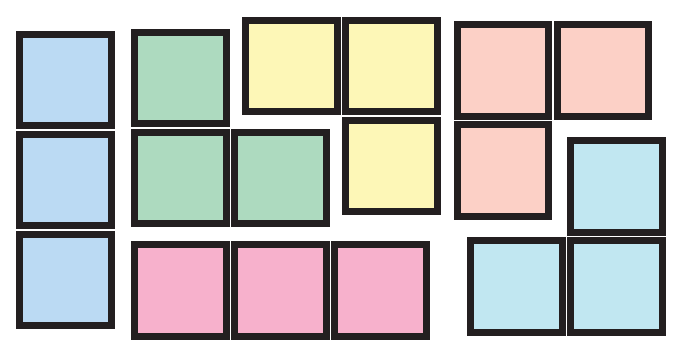
\includegraphics[scale=0.5]{img/pieces.eps}
\end{center}

Ce TP est fait pour être réalisé en équipe (2-4 membres) mais vous pouvez très
bien le faire tout seul, si vous en êtes capable (même si c'est moins marrant).
\\

\textbf{But du TP :} apprendre à utiliser \textbf{Git} à plusieurs et apprendre
les bases d'\textbf{XNA}.

\tableofcontents

\section{Création du dépôt Git et du projet XNA}

\noindent{\color{red} Si vous êtes bloqué à une étape, les assistants sont là pour vous
aider. Alors n'hésitez pas à leur demander.}

\begin{enumerate}
    \item Commencez par tous vous inscrire sur \url{https://bitbucket.org} ou
    \url{http://github.com} (mais tous au même endroit sinon ça va pas le faire). \\
    Ces deux sites permettent à des développeurs d'héberger leurs dépôts Git, et ce
    gratuitement.\\
    \textbf{Attention} : GitHub ne permet pas de faire de dépôt privé
    de base; il faut un compte étudiant. Préférez BitBucket si vous n'êtes pas
    quelqu'un d'opensource.\\

    {\color{red} \textbf{Attention} : \\Les étapes \textbf{2} et \textbf{3}
    sont faîtes par une seule personne. Choisissez là. Les autres regardent et
    l'aident.}\\

    \item L'heureux élu se rend sur le site que vous avez choisi et créé un
    nouveau dépôt (en général y'a un gros bouton pour ça, vous allez y arriver). \\

    \item Cette même personne créé un nouveau projet XNA sur VS.
\end{enumerate}

\% \textbf{TODO}: Corwin doit rajouter des étapes pour l'extension Git de VS
À la fin, ils sont tous sensés avoir le nouveau projet sur leur VS

\section{Principe du jeu}

\begin{center}
    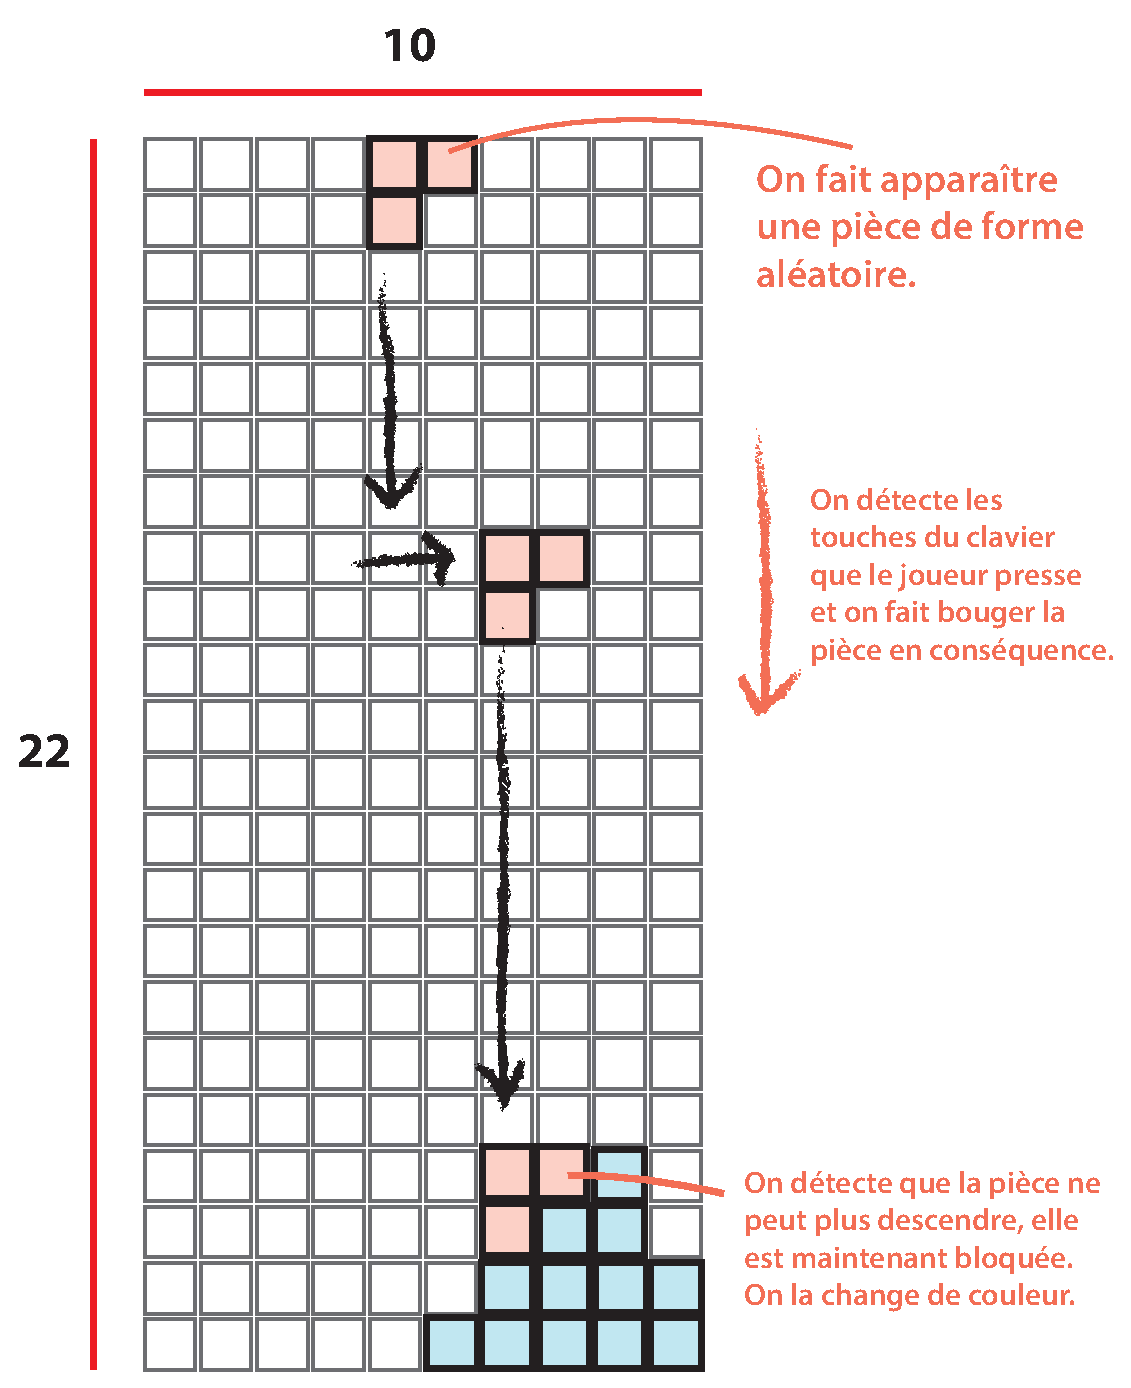
\includegraphics[scale=0.5]{img/game-explanation.eps} 
\end{center}

%

\end{document}

